\chapter{Creating and Meshing a curved pipe geometry in Salome for OpenFOAM}
\thispagestyle{empty}
\label{sec:chap11}
\newcommand{\LocCHelevenfig}{\Origin/CHAPTERS/chap11/figures}

This chapter deals with Creating a curved pipe geometry ( pipe bend ) using Salome and Meshing it.The curved pipe system is important in power plants and process industries. It is often important to predict flow field and temperature fields in the neighborhood of the mixing region in order to properly design the location of inlet pipes.

\section{Prerequisite}
The chapter assumes that the user has worked through the previous chapter on Salome Installation and has it running in his system

\section{Problem Description}

The problem to be considered is shown Schematically in Figure. The dimensions used here are in mm.We will use the bottom-up approach here. This approach means that you will first create some vertices, connect the vertices with edges and connect the edges. The only difference here is that wwe would be used a divided disc approach to create a face for the pipe which will be then extruded along the path to complete the 3D pipe.

\section{Procedure}

Start Salome by clicking the icon on your desktop. This will open up the Salome working window Figure, \ref{salome}. \newline

\begin{figure}[h]  
\centering
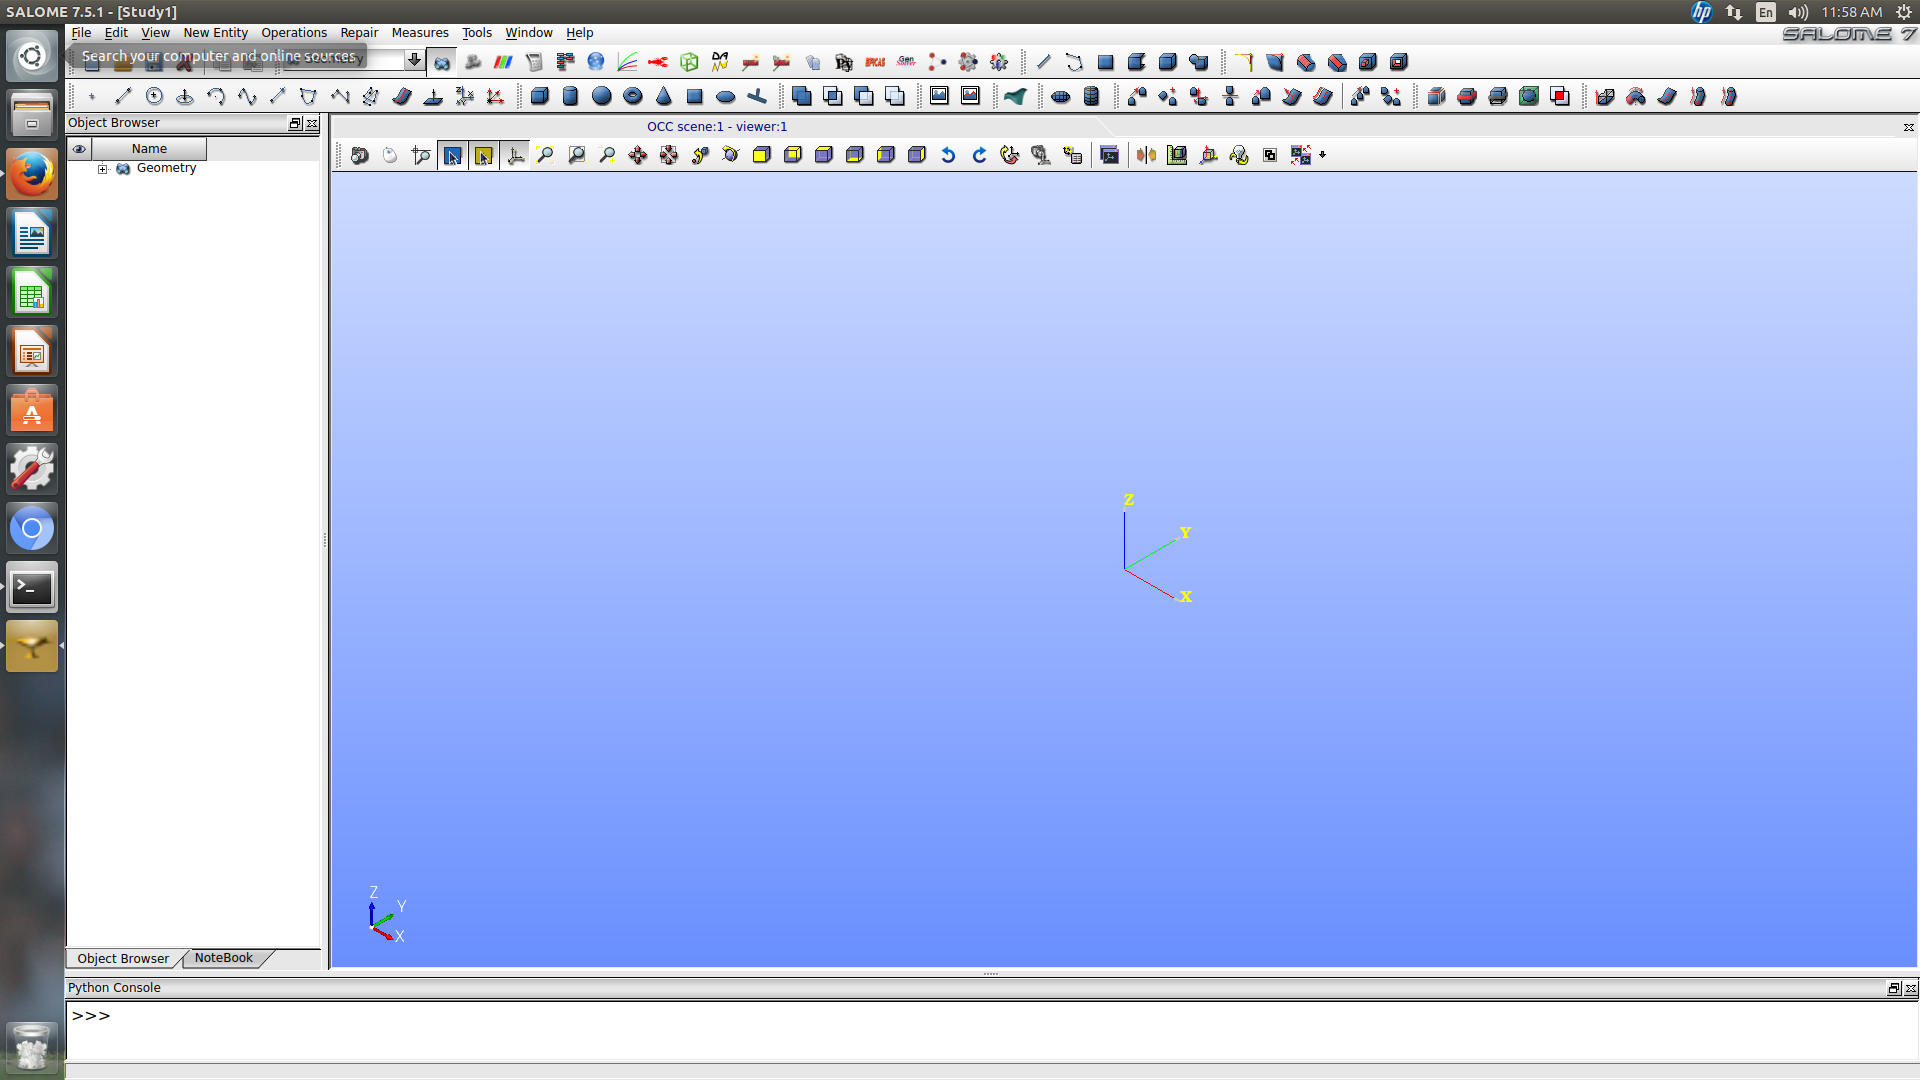
\includegraphics[scale=0.35]{\LocCHelevenfig/salome1.png}
\caption{Salome working window}
\label{salome}
\end{figure}

\subsection*{Active Module}

\begin{figure}[h]  
\centering
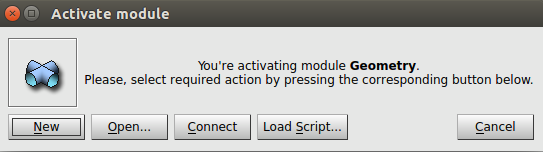
\includegraphics[scale=0.45]{\LocCHelevenfig/activate.png}
\caption{Activate module to open new file}
\label{activate}
\end{figure}

To create geometry we first need to select Geometry from the module drop down menu. We will open up a window which says Activate module,Figure. In this the user can Open a new window, Open an already created file , connect to different systems or Load an exsiting python script. Since we do not have an existing geometry we will create a new geometry here, so click on the New tab, Figure \ref{activate} . 

\subsection*{Geometry Properties}

\begin{figure}[h]  
\centering
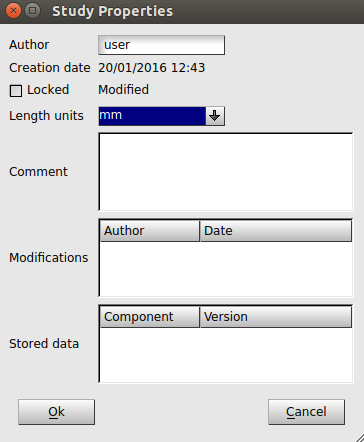
\includegraphics[scale=0.45]{\LocCHelevenfig/salome_prop.png}
\caption{Property table to set dimension}
\label{prop}
\end{figure}

After this on the top menu bar, click on File/Preference. This opens up the preference window where we can set the dimensions for our geometry, Figure \ref{prop}. Name of the Author can be the user. You can lock the dimensions for all your cases by clicking on the Locked buton below author. In the drop down menu besides Length, change it to mm. Other parts of the property panel can be kept default.

\subsection*{Geometry}

\begin{figure}[h]  
\centering
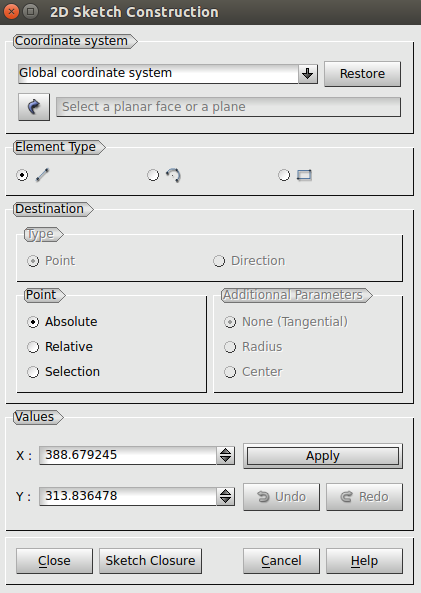
\includegraphics[scale=0.45]{\LocCHelevenfig/2dsketch.png}
\caption{2D Sketch construction window}
\label{point}
\end{figure}

To create geometry we will first create our base point. To do this launch the 2D Sketcher by clicking on the top menu \textit{New Entity/ Basic / 2D Sketch}. Enter the coordinates of the point of origin (0, 0) and click the Apply, Figure \ref{point}. Create the 1st Vertical segement using Line type element / Destination - Point/ Point - Absolute and enter the values (0, 30). We will now create an arc for our pipe bend, by Selecting the Element Type- Arc/ Destination - Direction/ Direction - Tangent and enter the values for Radius as -10 and Angle as 90 degree. The horizontal line can be drawn using Element type - Line / Destination - Direction / Direction - Tangent and enter the length for line as 30. Click on the close button. Do not click on the Sketch Closure button as this will join the starting point and the end point by a line.

\subsection*{DividedDisk}

\begin{figure}[h]  
\centering
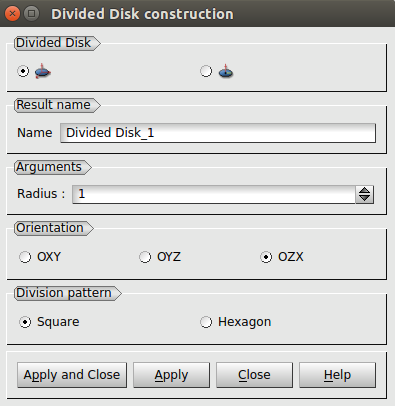
\includegraphics[scale=0.45]{\LocCHelevenfig/divideddisk.png}
\caption{Divided Disk Construction window}
\label{disk}
\end{figure}

We will now create a face for inlet of our pipe using Divided Disk object. It is a disk divided into blocks for easy hexahedral meshing. Two division patterns are available a Square pattern and a Hexagonal pattern. This can done by \textit{ New Entity/ Blocks / Divided Disk}. Divided Disk construction will open up, enter in this the Radius of the pipe as 1, orientation is the plane on which the disk will be built as OZX and the division pattern as square, Figure \ref{disk}. Click on Apply and Close.Final geometry will be as seen in the Figure \ref{disk1} 

\begin{figure}[h]  
\centering
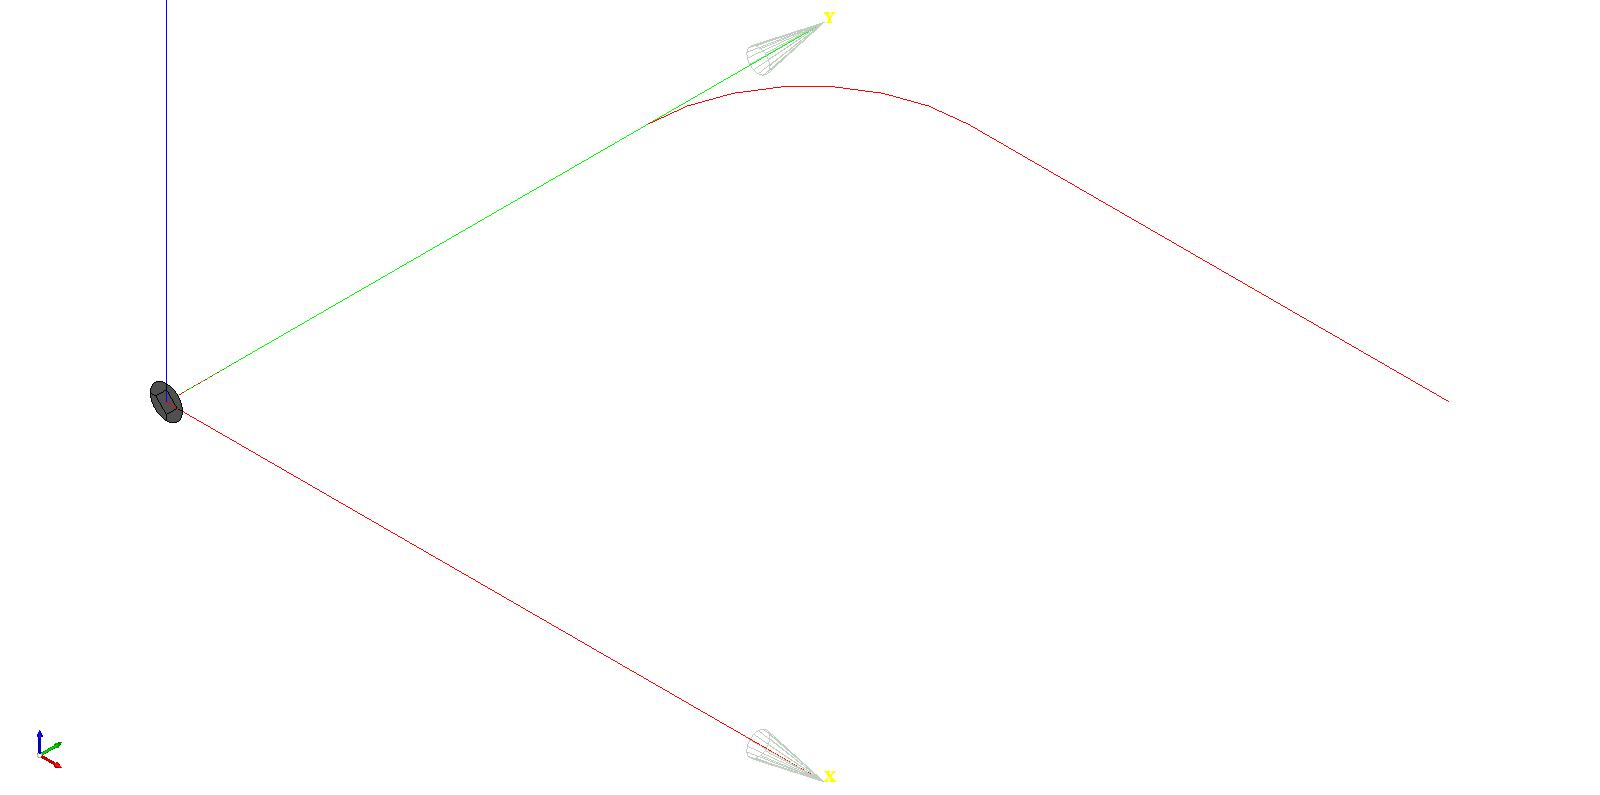
\includegraphics[scale=0.35]{\LocCHelevenfig/divideddisk1.jpg}
\caption{Inlet face using divided disk}
\label{disk1}
\end{figure}

\subsection*{Extruction}

\begin{figure}[h]  
\centering
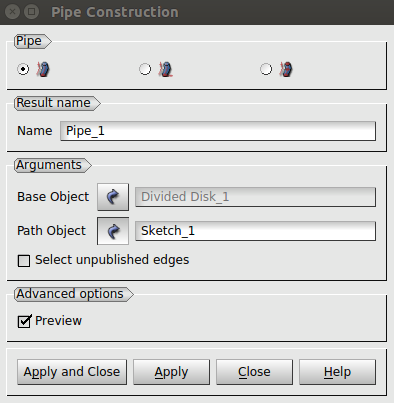
\includegraphics[scale=0.35]{\LocCHelevenfig/pipeconst.png}
\caption{Pipe Cnstruction window}
\label{pipeconst}
\end{figure}

\begin{figure}[h]  
\centering
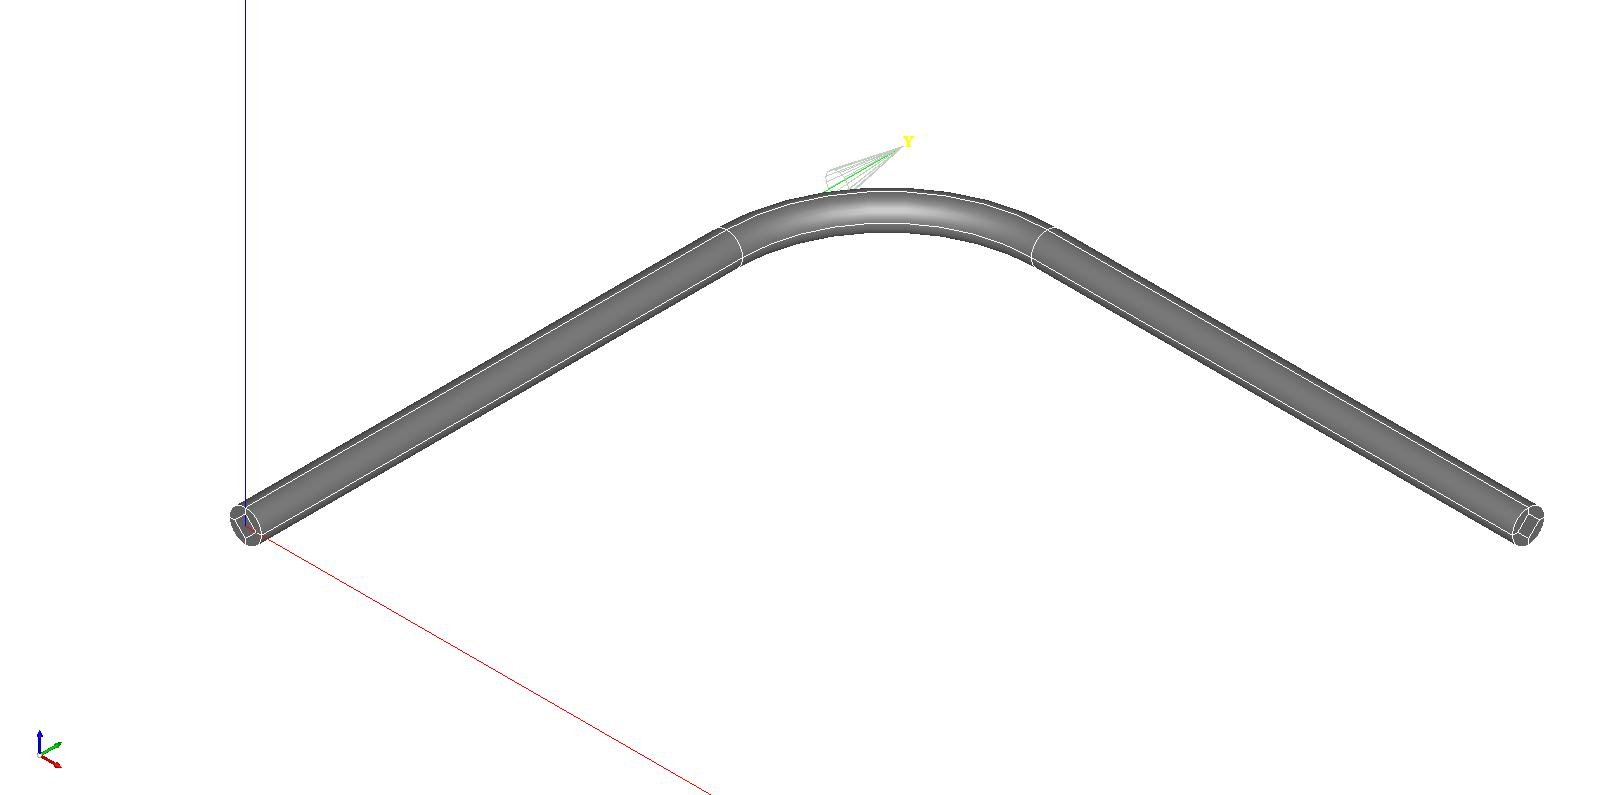
\includegraphics[scale=0.35]{\LocCHelevenfig/salome_pipe.jpg}
\caption{3D pipe bend}
\label{3dpipe}
\end{figure}

For construction of the 3D pipe we need to extrude the face created using divided disk along the curve generated earlier. Click on \textit{New Entity/ Generate / Extrude Along path}. In the Pipe constrution window name the pipe as Pipe-1, base object as Divided Disk-1 and the Patch Object as Sketch-1, Figure \ref{pipeconst}. Click Apply to close the window.3D bent pipe is now constructed as seen in the Figure \ref{3dpipe}.    

\subsection*{Explode}

\begin{figure}[h]  
\centering
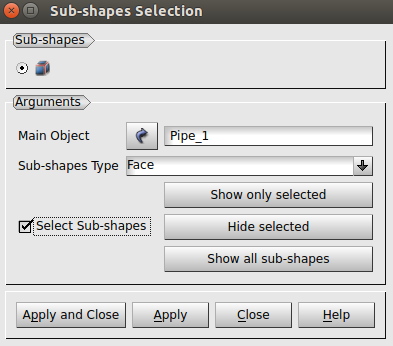
\includegraphics[scale=0.35]{\LocCHelevenfig/subshape.png}
\caption{Sub-Shape selection dialog box}
\label{subshape}
\end{figure}

\begin{figure}[h]  
\centering
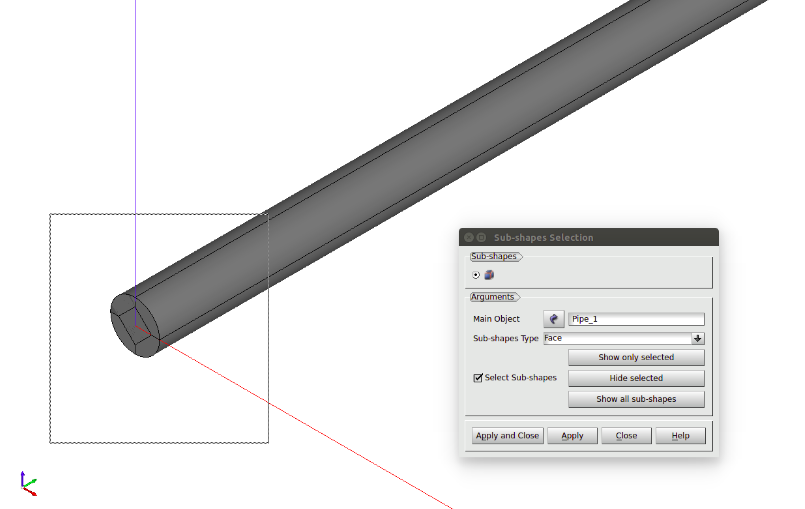
\includegraphics[scale=0.35]{\LocCHelevenfig/subshape_inlet.png}
\caption{Sub-Shape face selection for Inlet face}
\label{subshape_inlet}
\end{figure}

\begin{figure}[h]  
\centering
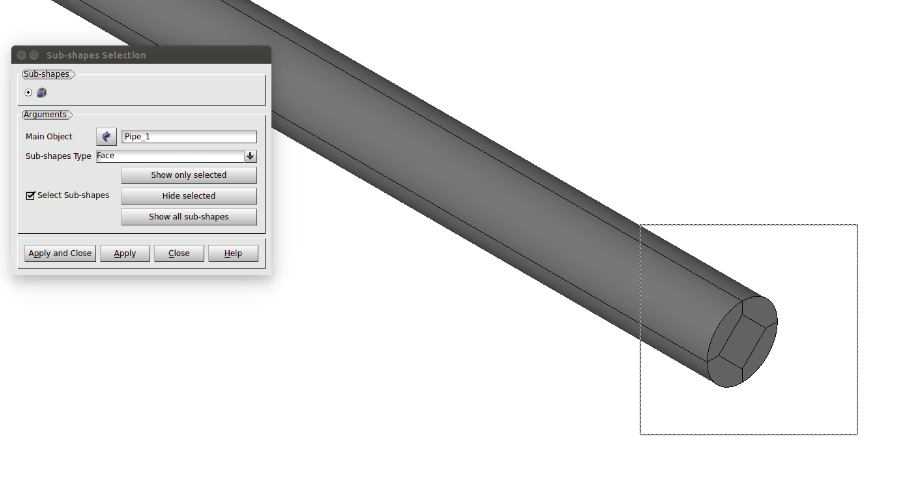
\includegraphics[scale=0.35]{\LocCHelevenfig/subshape2.png}
\caption{Sub-Shape face selection for Outlet face}
\label{subshape_outlet}
\end{figure}

To explode an object into sub-shapes in the Main menu slect \textit{New Entity / Explode}. This operation opens the sub shape selection dialog box. It is useful since we can extract the solid, face, edges, points needed to group. For our case , select the main object as Pipe-1, Sub-shape Type as Face. Also click on the Select Sub-Shape check box to select the required subshape, Figure \ref{subshape}. Now we will first select the inlet face first. To do this using the left click of the mouse drag your curser over the inlet face as seen in the Figure \ref{subshape_inlet}. The edges of the face would turn white. Now click on the Show only selected tab , to see the selected face and click Apply and Close.Repeat the procedure for outlet face as well.On the left hand side of the working window we can see the 10 faces under Object Tree structure. \newline

\begin{figure}[h]  
\centering
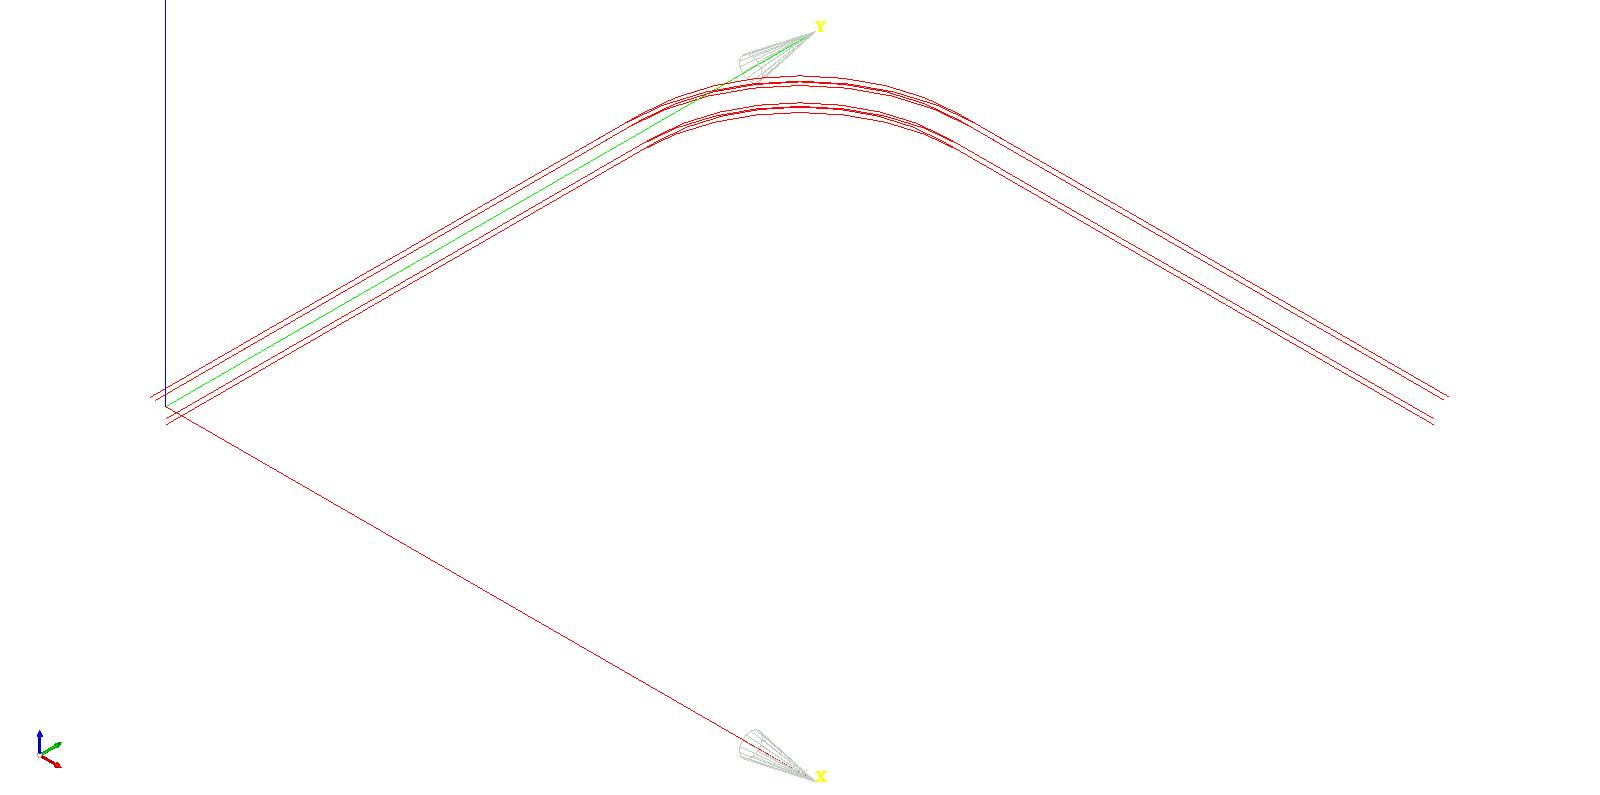
\includegraphics[scale=0.35]{\LocCHelevenfig/edges.jpg}
\caption{Exploded edges}
\label{edges}
\end{figure}

\flushleft We will also explode the edges along the flow direction. This is required since we need a finer mesh along the flow direction. Click on the \textit{New Entity / Explode} option. In the Sub-shape selection dialog box select the Main object as Pipe-1 and the Sub-shapes as Edges since we need to explode edges to group them. Select the Sub-shapes box and then Drag your right click mouse pointer over the inlet face and click on Hide Selected to hide the face as we want only the edges. Repeat this process for remaining faces. Finally drag the mouse pointer over edges as shown in the Figure \ref{edges} and click on Apply and Close. On the right hand side in Object browser tree we will see seperate 24 edges.

\subsection*{Groups}

\begin{figure}[h]  
\centering
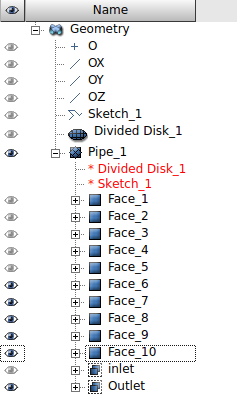
\includegraphics[scale=0.45]{\LocCHelevenfig/tree_salome.png}
\caption{Object browser tree}
\label{tree-salome}
\end{figure}

This operation allows creating groups on all selected shapes. Only the main shape of the geometry and Subshape needs to be selected. Click on \textit{New Entity/ Group / Create Group}. A Create Group window will pop-up. Under shape type select Face, name the group as Inlet, choose the main shape as Pipe-1. Select the first five faces (1-5) as subshape and Click on Add. Click Apply and Close to see the inlet group cerated in the Object tree browser. Repeat the same process for the outlet faces by selecting the faces (6-10) and name the group as Outlet, Figure \ref{tree-salome}. Now to group the edges along flow direction in Create Group dialog box select edges, Name the group as flow-direction, main shape as Pipe-1 and select the 24 edges exploded and Click on the Apply and Close button to create a group for flow-direction edges.This will help us in identifying the faces when we export the geometry for Simulation.

\section{Meshing Module}

\begin{figure}[h]  
\centering
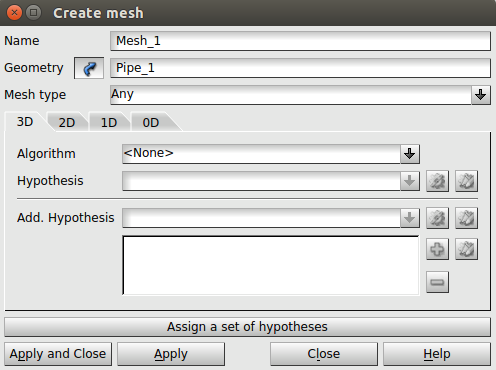
\includegraphics[scale=0.35]{\LocCHelevenfig/mesh.png}
\caption{Create mesh dialog box}
\label{edges}
\end{figure}

\begin{figure}[h]  
\centering
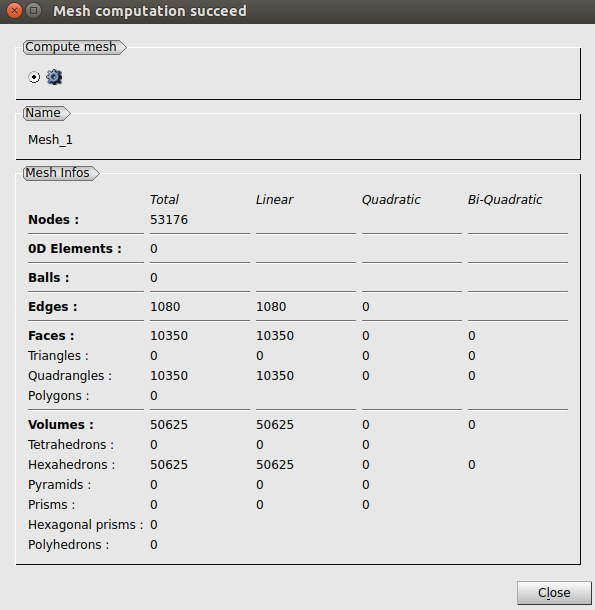
\includegraphics[scale=0.35]{\LocCHelevenfig/mesh_info.png}
\caption{Mesh information box}
\label{meshinfo}
\end{figure}

The goal of this module is to create meshes on the basis of geometrical models created or imported in the Geometry Module. It uses a set of meshing algoriths and their corresponding conditions (hypothesis) to compute meshes. Click on the Modules drop down Menu and change it from Geometry to Mesh. To mesh our geometry click on \textit{Mesh / Create Mesh}, this will open the Create Mesh dialog box, Figure . Name the mesh as Mesh-1, Select the geometry as Pipe-1 and click on the Assign a Set of hypotheses button to Select 3D: Automatic Hexahedralization. This will open up another dialog box , in this enter the Number of Segments as 15. Click OK to close this box and click on Apply and Close to close the create mesh box.Now in the Object browser tree rght click on Mesh-1 and selct Compute. This will mesh our geometry.A dialog box will appear at the end of Meshing providing the mesh information , Figure \ref{meshinfo}.\newline

\flushleft To save the Geometry, click on the File menu in the menu bar and click on Save As. Name the file as curved-geometry and the file format as .hdf ( a standard developed by Boeing and NASA in the aera of CFD ).

\section{Assignment}

As a practice assignment create a curved pipe having a radius of 1.5 mm and total length of 200 mm. Mesh the geometry and save it. 


